\documentclass{beamer}

% Use the provided theme
\usepackage{beamerthemetuw}

% Set title, author, date
\title{Rust meets Reality}
\subtitle{Usage, Community and Tooling}
\author{Mark Chimes}
\date{\today}

\begin{document}

% Title slide
\begin{frame}
    \titlepage
\end{frame}

% Outline slide (optional)
%\begin{frame}{Outline}
%    \tableofcontents
%\end{frame}

% Section 1
\section{Main Content}



\begin{frame}{Rust in Production - Do You Run Rust Code?} 
	\begin{block}{}

\begin{itemize} 
	\item \textbf{Firefox} 
	12\% of code. Migrated server push-notification architecture.
	\item \textbf{Rust-For-Linux Project} 
	Comprises 0.125\% (1/800th) of Linux kernel
	\item \textbf{Ripgrep} 
	Powers text search in VS Code
	\item \textbf{Dropbox}
	components of core file-storage system
	\item \textbf{Cloudflare}
	HTTP proxy (Pingora), DNS stack, DDoS 
	\item \textbf{Git} Added first Rust code a few days ago: 
	libgit-sys and libgit wrappers, and Rust Foreign-Language Interface
	\item \textbf{Ubuntu} plans to replace GNU utilities with Rust implementations
	(e.g. \texttt{ls, cp, find, diff})
\end{itemize} 
\end{block}
\end{frame} 

\begin{frame}{} 
\begin{center}
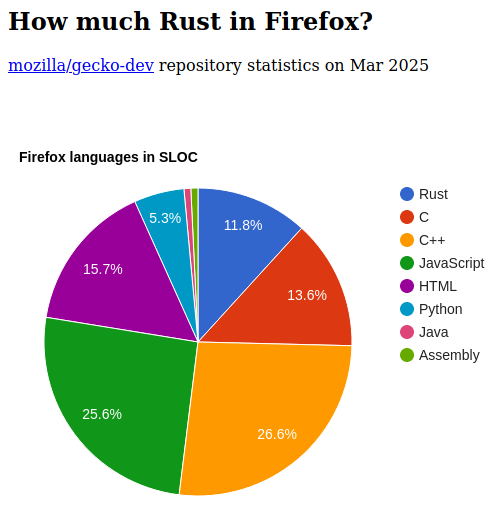
\includegraphics[scale=0.45]{rust-in-firefox}
\end{center}
\url{https://4e6.github.io/firefox-lang-stats/}
\end{frame} 

\begin{frame}{Openhub Rust Language Statistics} 

\begin{center}
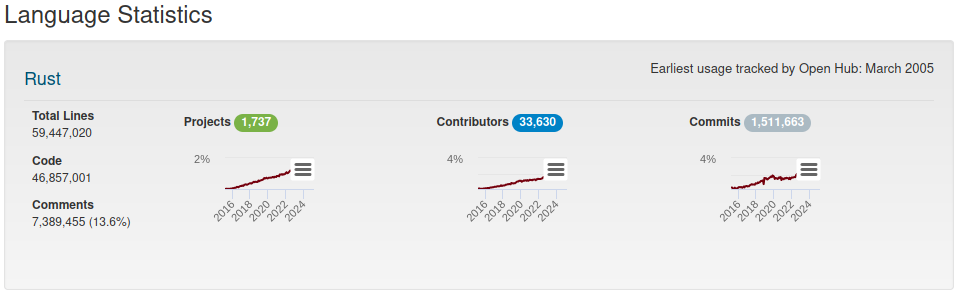
\includegraphics[scale=0.4]{openhub-statistics}
\end{center}

\url{https://openhub.net/languages/rust}


\url{https://madnight.github.io/githut/\#/pull_requests/2024/1}
(next page)

\end{frame} 

\begin{frame}{GitHut 2.0 - Github Language Stats } 
\begin{center}
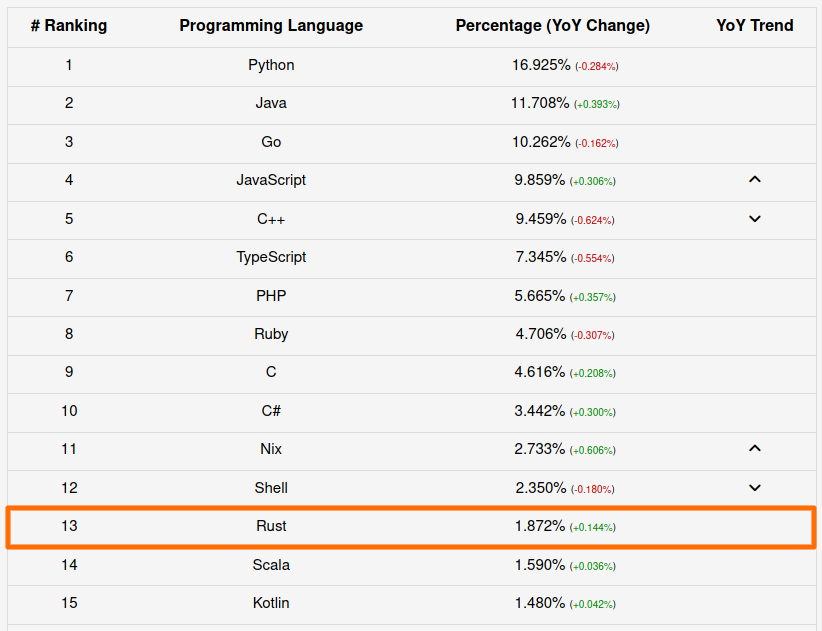
\includegraphics[scale=0.4]{githut-statistics}
\end{center}
\end{frame} 


\begin{frame}{Very Popular With Programmers} 

	\begin{block}{Stack Overflow Survey}

   	Rust is most ``admired", and 6th-most ``desired"

   \end{block}


    \begin{itemize}
    \item \textbf{Admired:} Already use, want to keep using
    \item \textbf{Desired:} Don't use yet, but want to
    \end{itemize} 
    
\end{frame} 

\begin{frame}{Popularity 2023} 
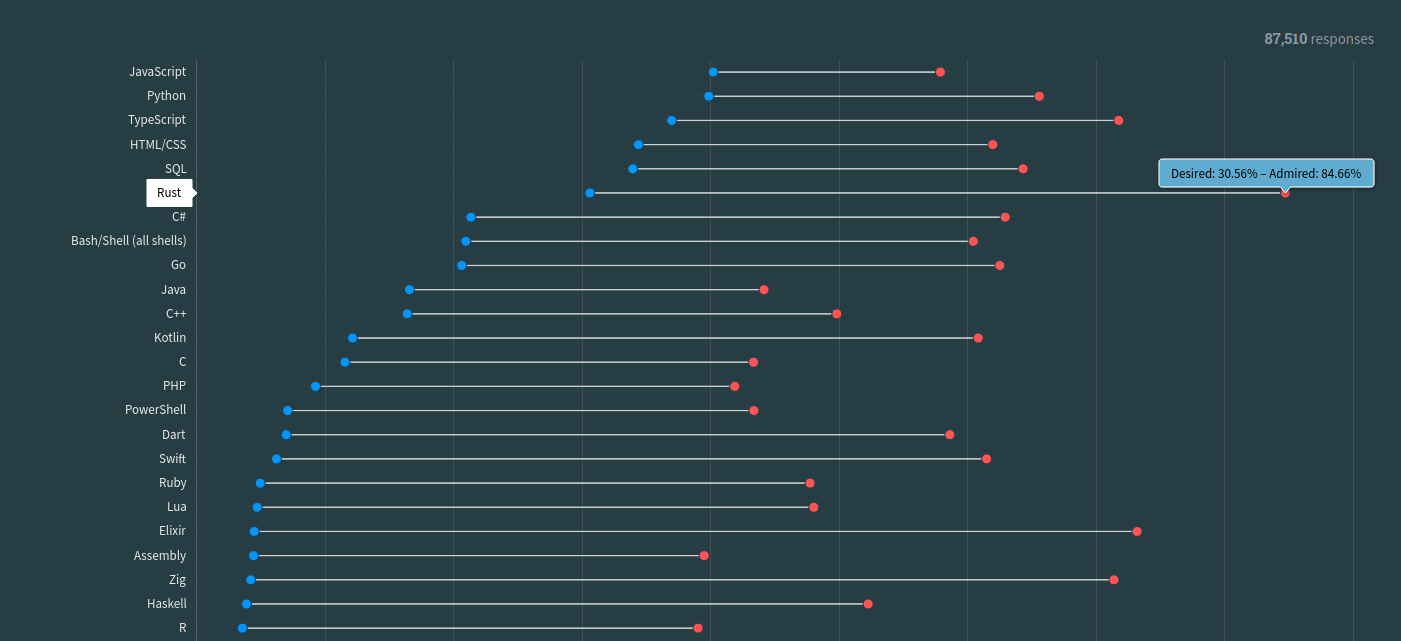
\includegraphics[scale=0.2]{desired-admired-2023}
Admired: 85\%
Desired: 31\%\\
\end{frame} 

\begin{frame}{Popularity 2024} 
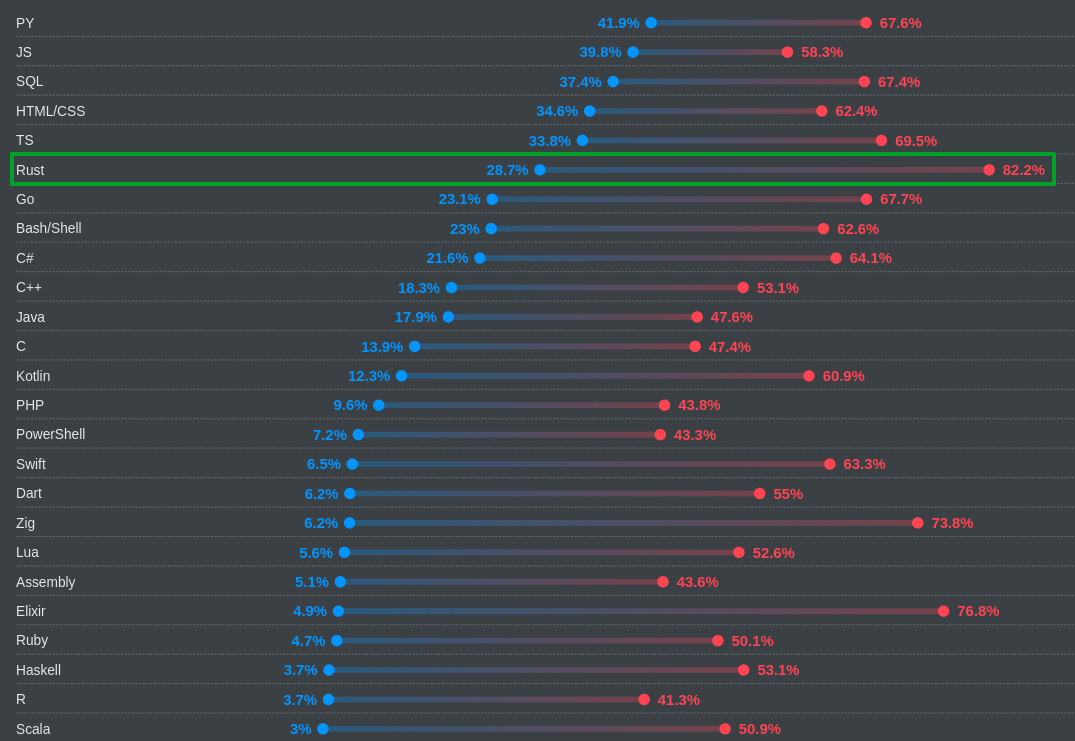
\includegraphics[scale=0.35]{desired-admired-2024}
\end{frame} 

\begin{frame}{History}
    \begin{itemize}
        \item[2006] Personal project by \textbf{Graydon Hoare} working at Mozilla
        \item[2009] Officially sponsored by Mozilla
        \item[2013] Hoare steps down, Rust Core Team formed
        \item[2014] Request for Comments (RFC) process introduced
        \item[2015] Rust 1.0 released
        \item[2016] Rust Mid-Level Intermediate Language (MIR) introduced
        \item[2022] Supported in Linux Kernel
        \item[2024] First Linux (network) drivers written in Rust accepted
    \end{itemize}
\end{frame}



\begin{frame}{Key Concept 1}
    Here is some content.
    \begin{itemize}
        \item Bullet point 1
        \item Bullet point 2
        \item Bullet point 3
    \end{itemize}
\end{frame}

\begin{frame}{Key Concept 2}
    Here is another slide.
    \begin{block}{Important Block}
        This is an emphasized block of text.
    \end{block}
\end{frame}

% Conclusion
\section{Conclusion}

\begin{frame}{Conclusion}
    \begin{itemize}
        \item Summary of key points
        \item Final remarks
    \end{itemize}
\end{frame}

\end{document}
